\section{Initial project plan}
Figure \ref{gantt1} shows a GANTT diagram that describes the progress  plan for this project, as it was defined at the beginning of the project. The analysis of requirements, abstract system design and a realization analysis are important parts of the project, as about half of the project time is dedicated to these tasks. The documentation of both the development process and the resulting software is an iterative process that is performed simultaneous to the other activities.
\begin{figure}[h!]
\centering
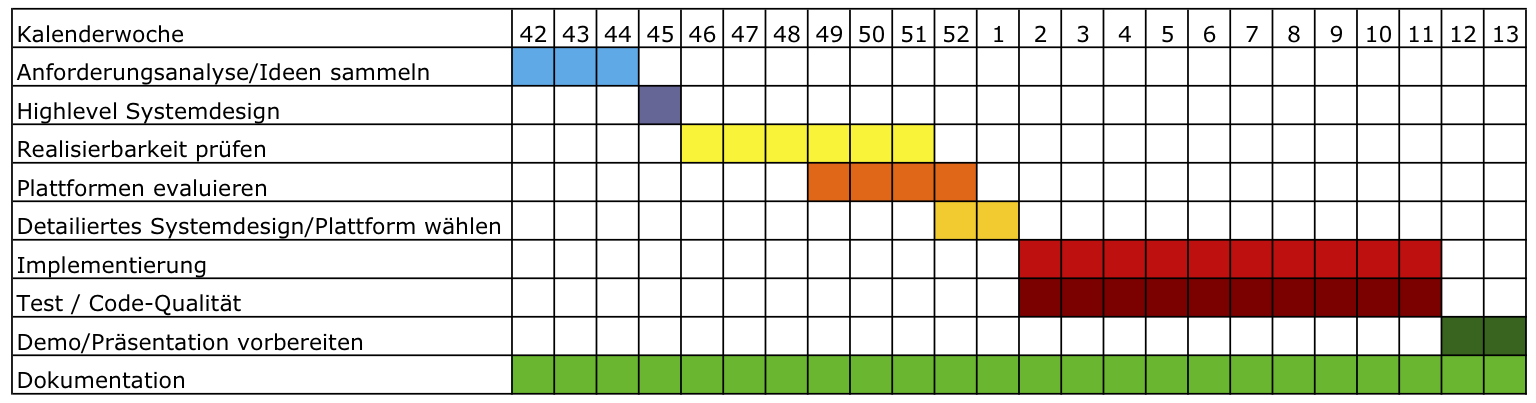
\includegraphics[width=16cm]{pics/gantt2.png}
\caption{Gantt diagram of the initial project plan (planing at project start)}
\label{gantt1}
\end{figure}
\section{Refined project plan}
During the development process it became obvious, that the initial project plan does not exactly reflect the amount of work necessary in the different work packages. Also milestones were introduced as a means to measure success in finer granularity than once at the end of every phase. Figure \ref{gantt2} shows the project plan as it was actually carried out. The key differences between the two plans are: 
\begin{itemize}
\item longer platform evaluation and realization evaluation phase
\item additional platform specific realization evaluation phase
\item longer overall development time, especially significantly longer implementation phase
\item break with the continuous documentation paradigm
\item introduction of milestones for the implementation phase
\end{itemize} 
\begin{figure}[h!]
\centering
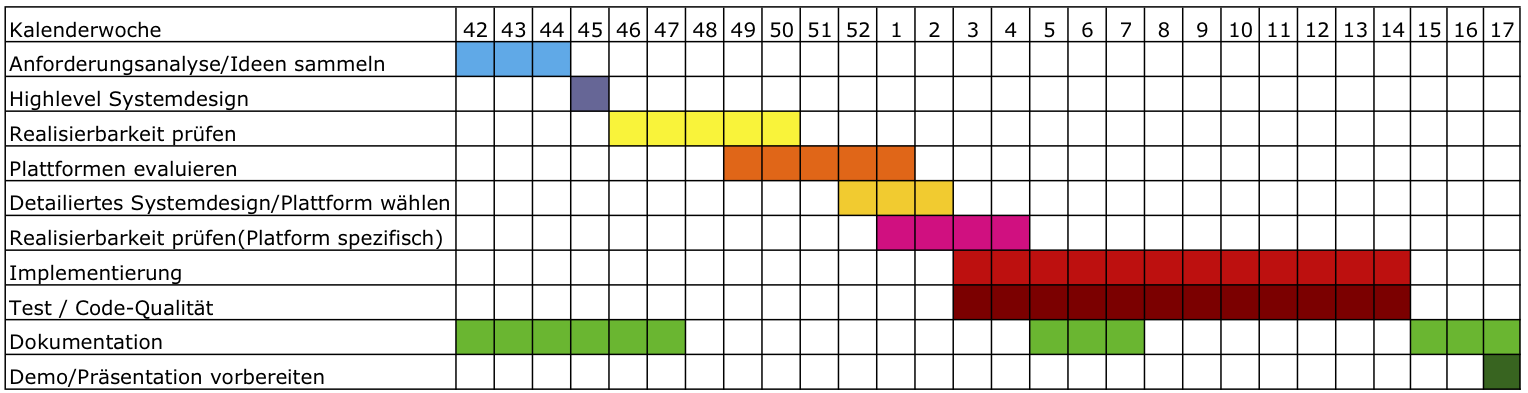
\includegraphics[width=16cm]{pics/gantt3.png}
\caption{Gantt diagram of the actually carried out project plan}
\label{gantt2}
\end{figure}
The following Milestones were introduces for the development phase:
\begin{itemize}
\item derive a OS specific system structure
\item install and get used to Android SDK
\item port Traveling Salesman routing engine to Android
\item solve biggest performance issues with routing engine
\item reverse-engineer the non-public Android calendar interface
\item finalize routing interface and implementation for Android
\item finalize calendar API
\item build system integration framework for Android OS, specifically  location and time triggered background tasks and user interaction
\item merge system parts into one unified application
\item determine performance of routing engine, identify bottlenecks and problems for future fixing
\item implement a structure to provide and manage dayplan information and checking/optimizing functionallity  
\item implement GUI for the task ''Generate and Manage Tasks''
\item implement GUI for the task ''Build and Manage day-plan''
\item implement background task ''optimize day-plan''
\item implement background task ''check day-plan for reachability of appointments''
\item write test-cases for the most important system parts (specifically the parts that could be reused in future projects)
\end{itemize}
The milestones are here not fixed to specific dates in the gantt diagram due to poor readability of the diagram. The order of the milestones reflects the order in which they were carried out.
